\documentclass[10pt]{article}
\usepackage{homework}

\begin{document}
\exheader{Molecular Photonics}

\exercise{1}
\begin{align*}
E^{ph}_{470nm} & \approx \frac{1242}{\lambda (nm)} \\
				& = \frac{1242}{470} \\
				& \approx 2.64 eV
\end{align*}
One electron-volt equals approximately 23.06 $\frac{kcal}{mol}$, thus
\begin{align*}
E^{ph}_{470nm} & \approx 23.06*2.64\frac{kcal}{mol}\\
				& = 60.94 \frac{kcal}{mol}
\end{align*}
One kilo-calorie equals approximately 4.19 kilo-Joules, thus
\begin{align*}
E^{ph}_{470nm}& \approx 60.94 * 4.19 \frac{kJ}{mol} \\
				& = 255.4 \frac{kJ}{mol}
\end{align*}
One reciprocal-centimeter equals approximately 12.399 meV, thus
\begin{align*}
E^{ph}_{470nm} & \approx \frac{2.64}{1.2399*10^{-4}} cm^{-1} \\
				& = 21293 cm^{-1}
\end{align*}

\exercise{2}
The oscillator strength is approximately given by
\begin{equation*}
f = 10^{-5} \bar{\nu} |er|^2
\end{equation*}
So from exercise one we have:
\begin{align*}
f  	&= 10^{-5} * 21293 * (1.6 * 10^{-19}* 3 * 10^{-9}) Ccm 
	& \approx Ccm
\end{align*}

\exercise{3}
The shape of the potential energy curve for a given state will be most strongly dictated by the position of the vibronic levels within that state.\\
The potential energy of a given vibronic level is proportional to the frenquency of oscillation of that level/for the given inter-atomic separation and the frequency of oscillation is inversely proportional to the mass of the vibrating particle. Accordingly, heavier atoms will `vibrate more slowly' at a given displacement from the equilibrium inter-atomic separation and their potential energy curves will be broader/more shallow than the ones of their lighter counterparts.
\begin{figure}
\begin{centering}
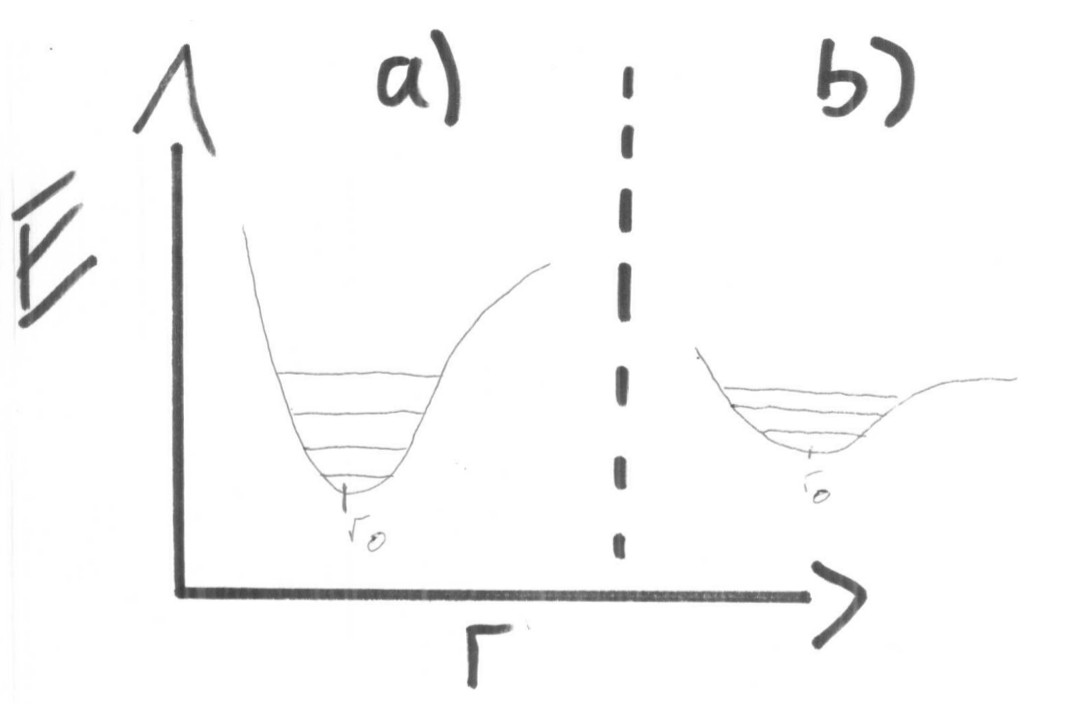
\includegraphics[width=0.5\textwidth]{f1}
\caption{Potential energy curves for diatomic molecules of a) light atoms and b) heavy atoms}
\end{centering}
\end{figure}

\exercise{4}
\sexercise{a}
The Born-Oppenheimer-Approximation states that nuclear as well as electron motion and spin can all be treated seperately from eachother. Because nuclei are very heavy compared to electrons, the latter will move much faster. The Frank-Condon principle translates the same idea to (UV-VIS) absorption and emission spectra: a given electronical transition will be more favourable if the initial and final nucleic positions are more similar.\\
\begin{figure}[!h]
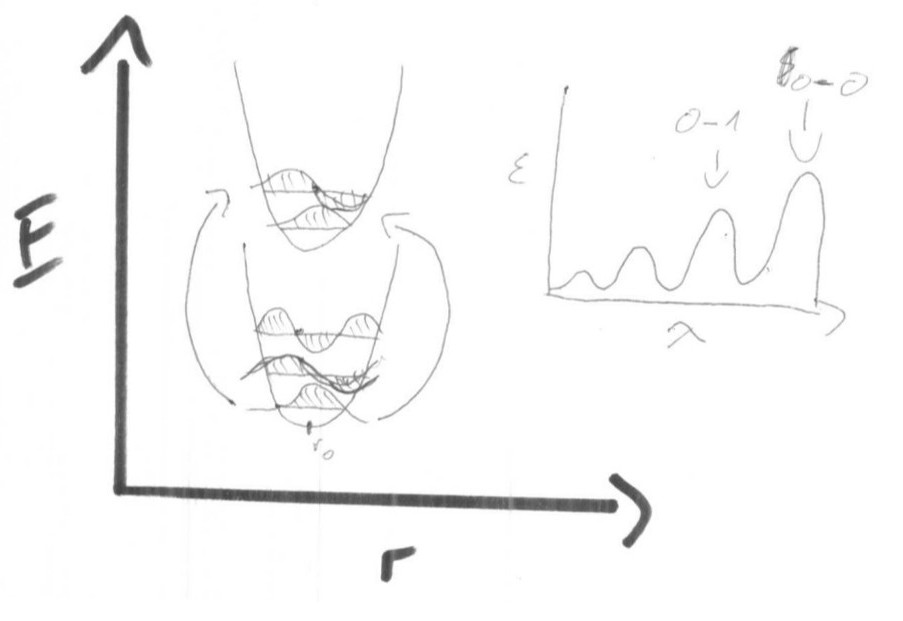
\includegraphics[width=0.45\textwidth]{f2a}
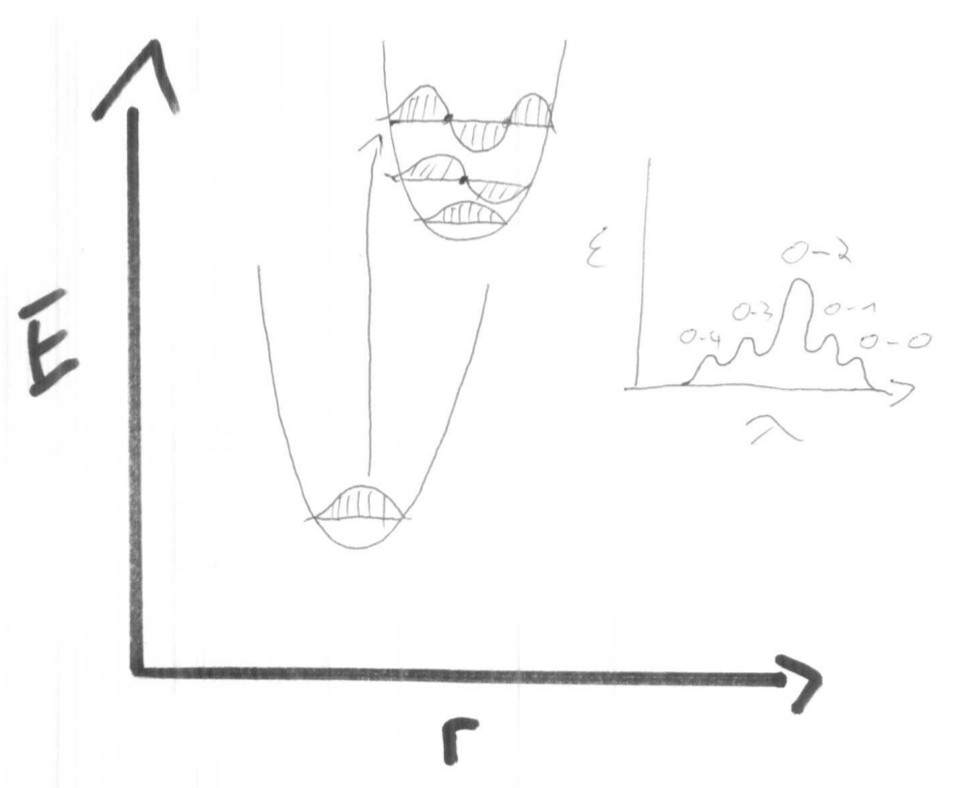
\includegraphics[width=0.45\textwidth]{f2b}
\caption{Potential energy curves for transitions in a) rigid and b) flexible pi-systems. The inlet gives corresponding, schematic absorption spectra.}
\end{figure}
In a very ridgid $\pi$-system, the nucleic position will be almost identical for the ground and excited states, whereas flexible systems allow for relaxation-motion of the nuclei to minimise the energy of the excited state. If you take into account overlap of the wavefunctions of their vibronic levels this will (\emph{ideally}) lead to a symmetrical distribution of the transitions peaks around the strongest, central peak in flexible systems, whereas rigid systems will show peaks properly ordered by the energy required for the transition
\sexercise{b}
The spectra will `smoothen out' because the solvent-molecule interaction introduces many energy-levels in between the vibrational levels

\exercise{5}
A given transition will (always) be more probable/efficient, when there is high overlap between the wavefunctions of the initial and the final state of the transition, i.e. when the square of the overlap (Frank-Condon-)integral is closer to 1. The preceding statement is true for radiative as well as radiationless transitions.
\begin{figure}[!h]
\begin{centering}
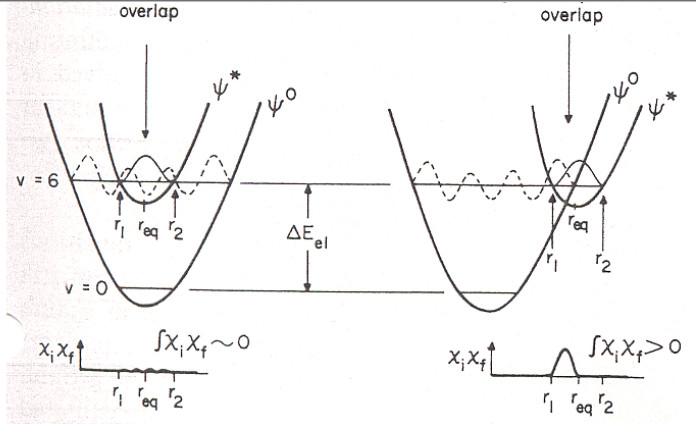
\includegraphics[width=0.45\textwidth]{f3}
\caption{Potential energy curves for left: in-effective and right: effective radationsless transition. Figure taken from the lecture-slides.}
\end{centering}
\end{figure}

\exercise{6}
Let us look at the simple aromatic molecules benzene, napthalene and anthracene first. Their $S_1$ transition-dipole should be identical in every case, because it is perpendicular to the molecule's long axis. The $S_2$ transition-dipole will be along the long axis and thus increase with the length of the aromatic. Perylene can be seen as two crossed anthracenes whose dipoles will add so it should have an even greater transition dipole than anthracene. The last molecule is already charged and contains the strongly electronegative species oxygen and thereby contains a ground-state dipole to begin with. Its transition-dipole should thus be the greatest of the five molecules.

\end{document}
